\documentclass[12pt, a4paper]{article}

\title{\textsc{Intro. To Computer Networks}\\Lab 1 Report}
\author{110062219 翁君牧}
\date{\today}

\usepackage{xeCJK}
\usepackage{float}
\usepackage{amsmath}
\usepackage{amssymb}
\usepackage{caption}
\usepackage{subcaption}
\usepackage{tikz}
\usepackage{pgfplots}
\usepackage{listings}
\usepackage{hyperref}
\usepackage{booktabs}
\usepackage{inputenc}
%\usepackage{biblatex}
\usepackage{longtable}

\setCJKmainfont{Songti TC}
\setCJKsansfont{Heiti TC}

\newfontface\ccpl{Cascadia Code PL}

\lstset{
	breaklines=true,
	basicstyle=\ttfamily,
}

\definecolor{nthu}{HTML}{7F1084}

\begin{document}

\maketitle

\tableofcontents

\section{建置與執行}

使用 \texttt{unzip} 指令解壓縮上傳至 eeclass 之檔案後,將得到一個目錄,切換為 working directory, 當中包含以下內容:

\begin{description}
\item[\ttfamily README.pdf] 即本 report.
\item[\ttfamily Makefile] 詳見以下說明。
\item[\ttfamily src/] 原始碼。
\end{description}

\texttt{Makefile} 預設將以 \texttt{gcc} 編譯 \texttt{src/} 下所有 \texttt{*.c} files 為 object files 至 \texttt{obj/} 中,並將所有(其實後來才發現只有一個)objects 連結為 binary file \texttt{a.out}. 此時完成建置後,即可以 \texttt{./a.out} 執行,如 Figure \ref{fig:screenshot}.

\begin{figure}[htbp]
\centering
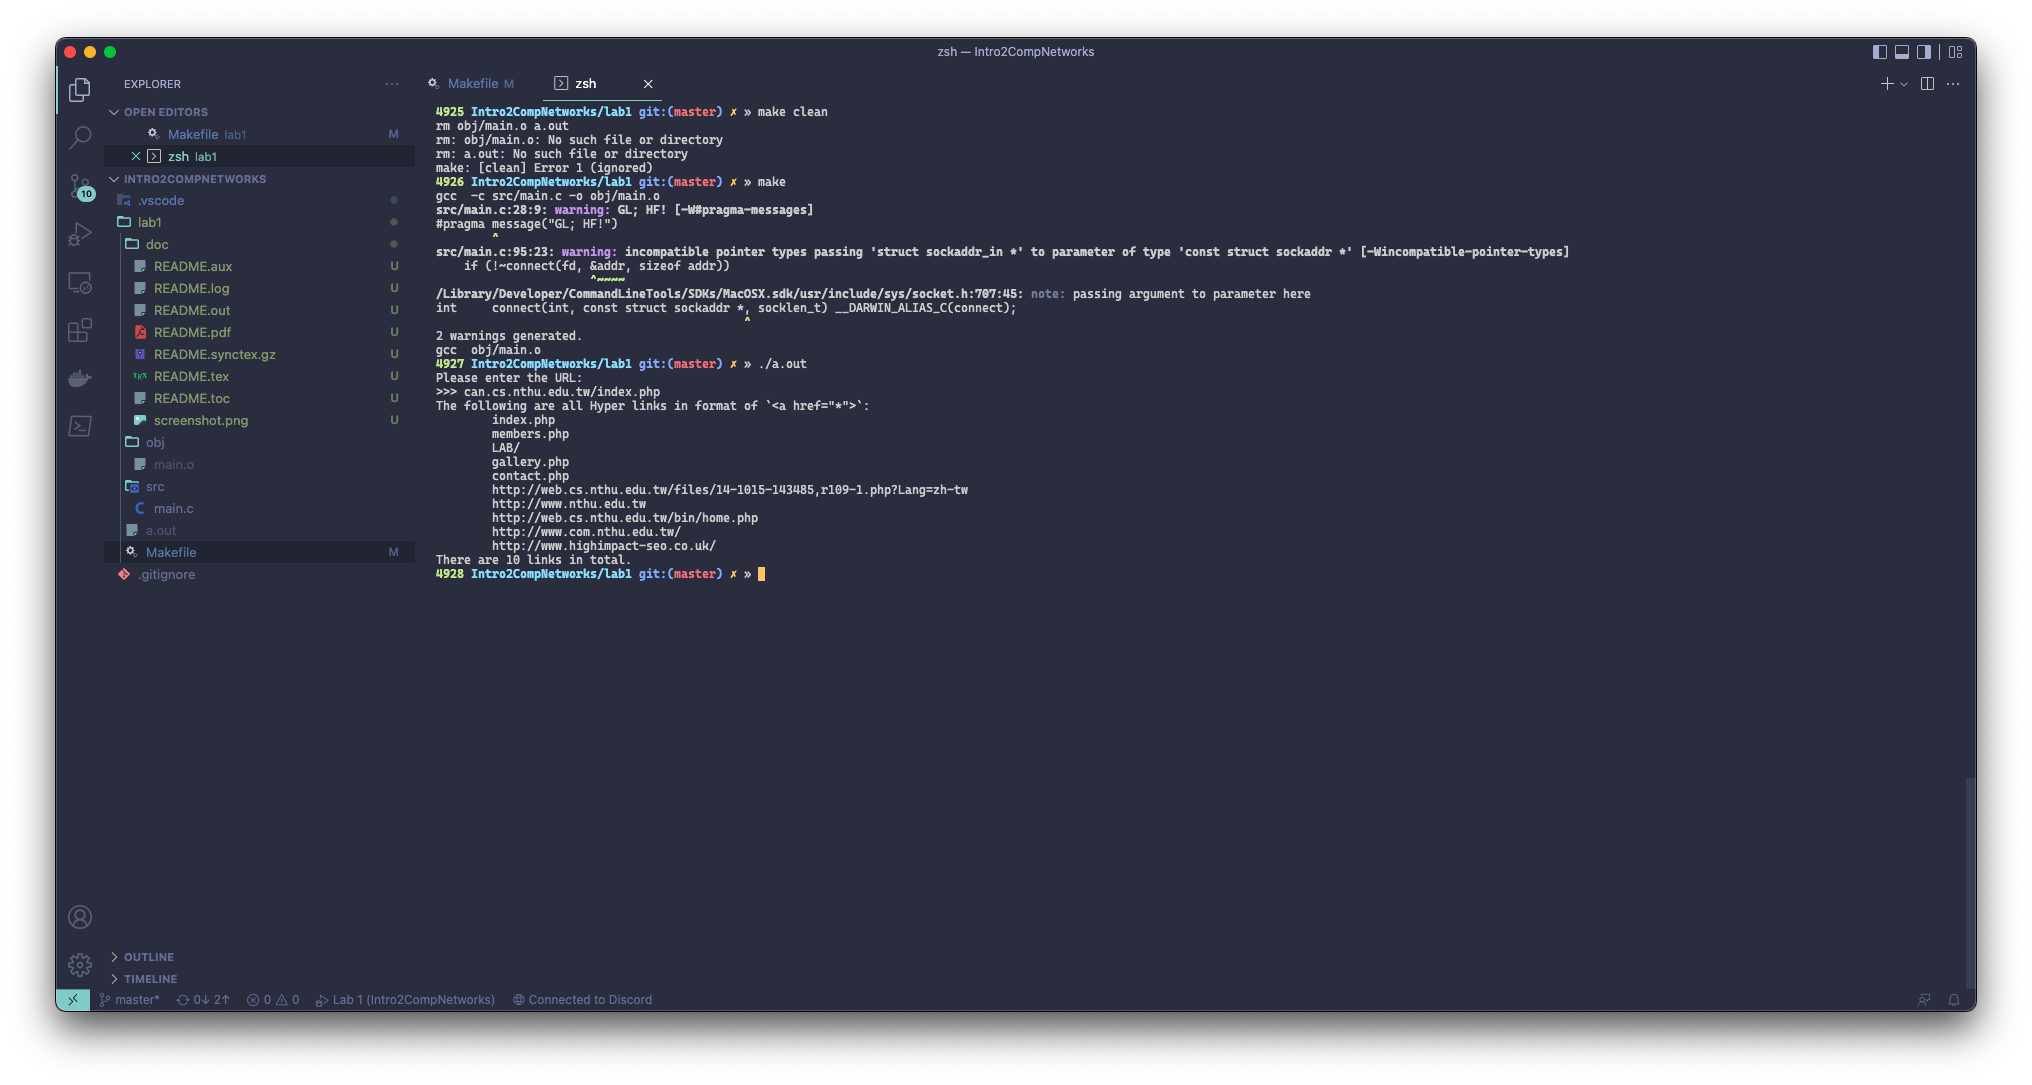
\includegraphics[width=\linewidth]{screenshot}
\caption{Screenshot of Execution}
\label{fig:screenshot}
\end{figure}

另外還提供兩種 targets \textsf{nevikw39}, \textsf{debug}. 前者在編譯時期將有更多警告以及提示訊息,後者則更會在執行時期於 \texttt{stderr} 以黃字輸出讀入的 host, path, 預計發出的 request, 收到的 buffer 的內容及大小等偵錯訊息並檢查越界存取、 Undefined Behaviors 等。

假若要直接以 \texttt{gcc} 編譯程式亦不難,因為這次 lab 最終只有 \texttt{src/main.c} 一份原始碼。

\section{設計}

如同前述,本次 lab 僅有一個 source code file, 而其主要可以分成 macros 以及四個部分。

\subsection{錯誤處理}

對於錯誤處理以及偵錯訊息,我採用 macros 的方式來定義。當在 \texttt{main()} 中遇到錯誤時,以紅字在 \texttt{stderr} 印出有關 line number, \texttt{errno} 所代表的錯誤訊息等。

\subsection{輸入}

程式執行起初,首先提示使用者輸入 URL \textit{(Unified Resource Link)}, 並假定輸入符合 \texttt{host(/path)} 的格式。我另外實作一個 function 以將 URL 分割為 $host$, $path$. 首先找到首個 `\texttt{/}', 並將前半段作為 $host$, 後半段作為 $path$; 假若未找到,則將整個 URL 當作 $host$, 並將 $path$ 定為 `\texttt{/}'.

\subsection{連線}

這個部分就是這次 lab 的核心 --- \textsf{Socket} programming. 具體流程則又可以細分為五步:

首先嘗試以 \texttt{socket()} 開啟一個 \textsf{IPv4} family, \textsf{Stream} \textit{(sequenced \& reliable)} type 與自動 protocol 的 \textsf{Socket} file descriptor. 接著,利用 \texttt{<netdb.h>} 中的 \texttt{gethostbyname()} function 將 hostname 以 system call 求得其 address. 再來就可以呼叫 \texttt{connect()} 嘗試建立 \textsf{TCP} 連線。

然後,我們就將 $host$, $path$ 填入以下的 request template:
\begin{quote}
\ttfamily
GET $path$ HTTP/1.0{\ccpl\itshape␍␊}\\
Host: $host${\ccpl\itshape␍␊}\\
Connection: close{\ccpl\itshape␍␊}\\
{\ccpl\itshape␍␊␍␊}
\end{quote}
其中,{\ccpl␍}, {\ccpl␊} 分別代表 carriage return (`\texttt{\textbackslash r}'), line feed (`\texttt{\textbackslash n}'). 而送出 \textsf{HTTP GET} request 則依賴於 \texttt{send()} function.

最終,我們以 \texttt{do-while} loop 搭配 \texttt{recv()} function, 持續接收到 buffer 直到不再有可讀的訊息。

\subsection{分析}

此部分則是一般程式的重要部分,parse, process 接收到的資料,尋找網頁上所有符合格式的超連結。想要現在有個 pointer / sweep line 指向 stream 的首端,我們向後搜尋 ``\texttt{<a href="}'' 的位置,假若資料合法且成功找到,則至下一個 `\texttt{"}' 前的字串即為所求的超連結。重複以上過程,直到遍歷完整個 buffer.

\subsection{釋放}

\texttt{free()} 掉一些動態配置的記憶體,並以 \texttt{<unistd.h>} 中的 \texttt{close()} function 關閉 \textsf{Socket}.

\section{心得}

約莫國中的時候曾經自己借書回來在 Windows 上以 \textsf{WinSock} API 撰寫一些很簡單的小程式。現在對於細節當然早就忘光,不過大致的概念像是 \texttt{socket()}, \texttt{bind()}, \texttt{connect()} 等 function 是還有一點印象。

實作上遇到最大的挑戰是在接收的時候。助教的 tutorial 是以 \texttt{send()} 傳送請求,以 \texttt{read()} 接收回覆。但根據我撰寫一些通訊相關的程式 (e.g., MPI \textit{(Message Passing Interface)}, \textsf{InfiniBand} RDMA \textit{(Remote Direct Memory Access)}) 的經驗,通常 \texttt{send()}, \texttt{recv()} 是一對而 \texttt{write()}, \texttt{read()} 則是另一對。原本我是宣告一個夠大的 buffer 只呼叫一次 \texttt{recv()} 就希望可以讀取全部,但執行後發現雖然有時可以完整得到 response, 但更多時候是有遺漏的。有嘗試給予 \texttt{recv()} \texttt{MSG\_WAITALL} 的 flag, 效果卻不彰。進一步查看接收到的長度,發現往往只有 1492 bytes, 而這個數字似乎與 MTU \textit{(Maximum Transmission Unit)} 有關。最終,我才採用 \texttt{do-while} loop 持續接收直到長度為 0. 這部分感覺還可以再優化記憶體,既然都用 loop 了可以有需要才 \texttt{realloc()}.

另一方面,一開始我以為需要找出所有 anchor tags 的 hyper links, 但 C 沒有內建的 \textsf{HTML} parser 而 \textsf{regular expression} 在 C 的支援也不熟悉。看了討論區之後,才知道我們僅需要列出型如 \texttt{<a href="*"></a>} 的 hyper links, 因此 \texttt{<string.h>} 中的 \texttt{strstr()}, \texttt{strchr()} functions 即足矣。

\subsection{跨平台可移植性}

十一日那週末我回到家中,在 Windows PC 上的 WSL \textit{(Windows Subsytem for Linux)} 直接開發,完成到處理 MTU 的部分。回到 Apple M1 Mac mini 上,同樣的程式碼不論以 bult-in \texttt{clang} 或 \texttt{gcc-12} installed from \textsf{Homebrew} 皆會發生 runtime error. 後來才找到原因出在讀入 URL 時,因為我使用 ``\texttt{\%ms}'' format specifier 來讓 \texttt{scanf()} 根據字串大小自動動態記憶體,\textsf{macOS} 的 \texttt{libc} 不支援卻編譯得了,導致執行時期 URL 什麼都沒讀到就被 splited.

而期中考時助教有再次強調程式碼必須可以在給定的虛擬機中運行,\textsf{Ubuntu} 的版本為 20.04. 我完全可以理解助教的考量。印象中我的 WSL 還停留在 \textsf{Ubuntu} 18.04, 可以執行虛擬機的 \textsf{Intel MacBook Pro} 的硬碟也已經被 \textsc{Logic Design Lab} 所需的 \textsf{Vivado} 用的 \textsf{Ubuntu} 22.04 幾乎耗盡。因此,我還是在 MacBook 以及 \textsf{Ubuntu} 22.04 VM 中編譯並成功執行,如 Figure \ref{fig:screenshot_ubuntu}.

\begin{figure}[htbp]
\centering
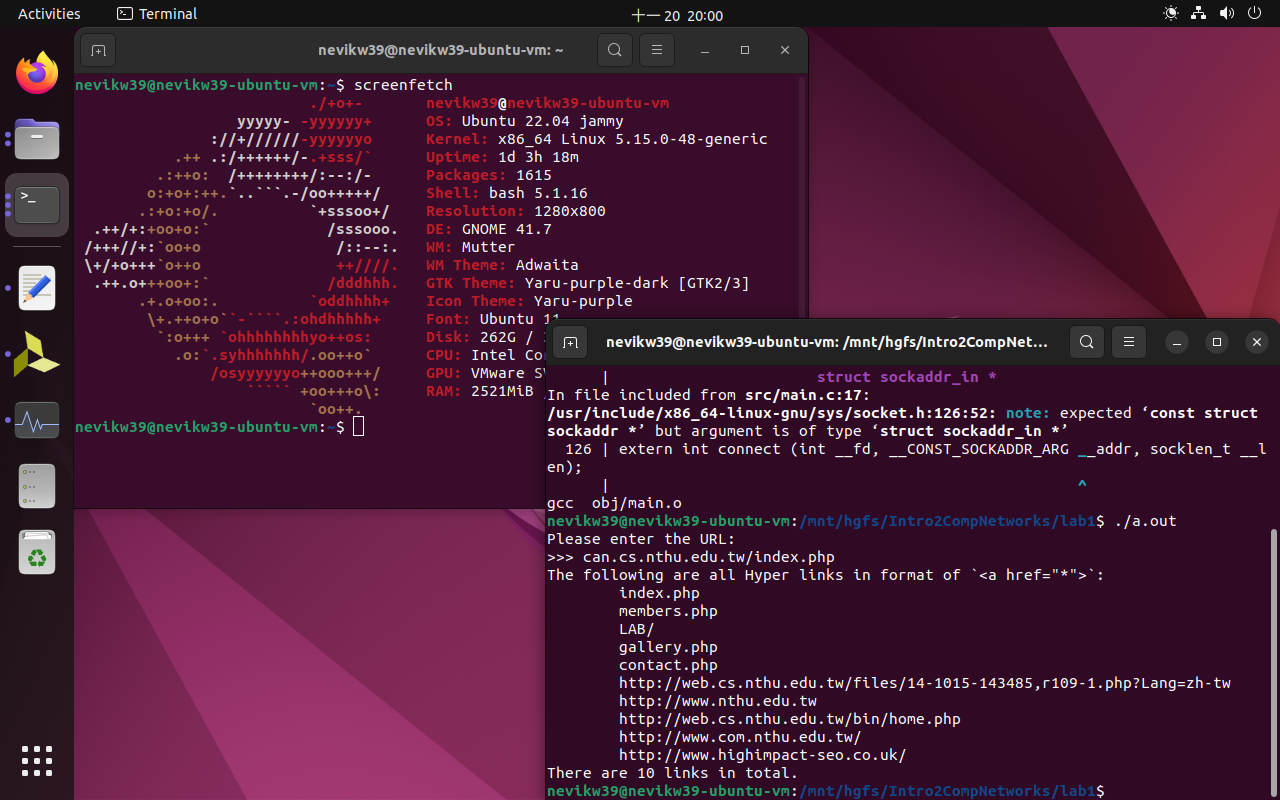
\includegraphics[width=.795\linewidth]{screenshot_ubuntu}
\caption{Screenshot of Execution on \textsf{Ubuntu} 22.04 VM}
\label{fig:screenshot_ubuntu}
\end{figure}

理論上 \textsf{Socket} 跨平台可移植性應該不會太差,畢竟 \textsf{macOS} 是衍生於 \textsf{POSIX}-compliant 的 \textsf{FreeBSD}, 而且現今的 \textsf{Socket} API libraries 大多是源於 \textsf{BSD Socket}. 我這次確實是遇到一些問題了,但主因是我使用了一些不在標準當中的語法,這裡是需要多加小心。

\subsubsection{Updates}

上網查到 \textsf{Ubuntu} 20.04 內建的 \texttt{gcc} 版本為 9.3.0. 因此我登入到國網中心的超級電腦\textbf{台灣杉三號},上面最接近的版本為 9.4.0.

此外,我也特別到資電館的電腦教室 328, 發現那裡的 \textsf{Ubuntu} 剛好是 20.04. 在這兩個額外環境下,我的程式也都能順利編譯並執行。因此,我有信心可以在助教的 VM 運行。

\begin{figure}[H]
\centering
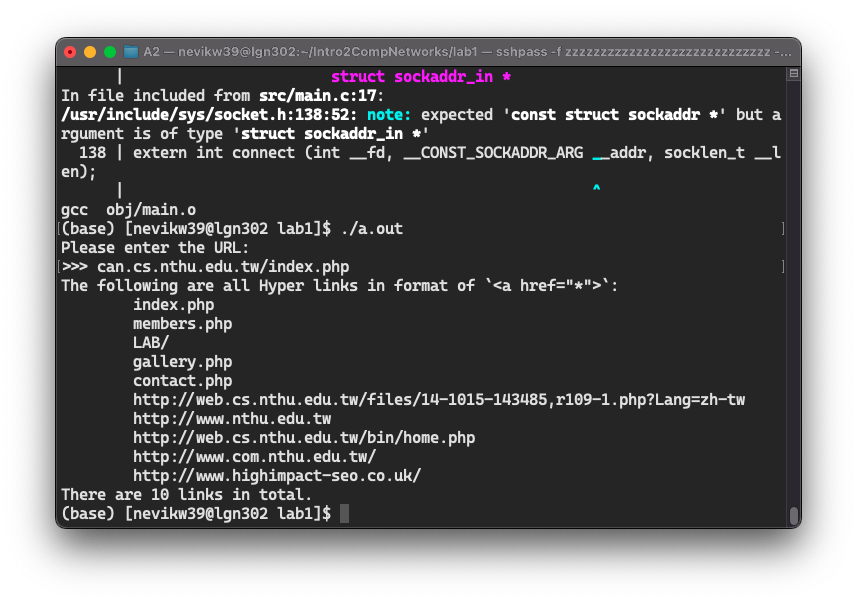
\includegraphics[width=\linewidth]{screenshot_twnia3}
\caption{Screenshot of Execution on \textbf{Taiwania 3}}
\label{fig:screenshot_twnia3}
\end{figure}

%\pagebreak

\begin{table}[htp]
\caption{Testbed (in Test Order)}
\centering
\begin{tabular}{c|c|c|c}
OS & Arch. & Compiler & Note \\\hline
Ubuntu 18.04 & x86-64 & GCC 10 & WSL 2 \\
macOS 12.4 & AArch64 & Apple clang 13.1.6 \\
macOS 11.6.4 & x86-64 & Apple clang 12.0.5 \\
Ubuntu 22.04 & x86-64 & GCC 11.2.0 & VM \\
CentOS 7.8.2003 & x86-64 & GCC 9.4.0 \\
Ubuntu 20.04 & x86-64 & GCC 9.3.0 & not VM \\
\end{tabular}
\label{tab:testbed}
\end{table}

\section*{Acknowledgements}

I thank to \textsf{National Center for High-performance Computing} \textit{(NCHC)} for providing computational and storage resources.

\end{document}
